\scanpage{121}


6) Supposons maintenant que $C$ soit une catégorie \deleted{additive}\inserted{abélienne} $k$-linéaire ($k$ un corps) munie d'un foncteur fidèle exact $F:C\handwritten{\to}\mathrm{Modf}(k)$, de sorte que $C$ s'identifie à la catégorie des représentations \deleted{d'un}\inserted{(continues)\handwritten{\begin{tikzpicture}[x=.55cm,y=.55cm,baseline=-.2ex]\draw (0,-.23) .. controls (.04,-.04) and (.14,.05) .. (.38,.05)--(1.8,.06) .. controls (2,.07) and (2.12,.2) .. (2.12,.42);\end{tikzpicture}}} finies d'une algèbre profinie $U$ sur $k$\inserted{(associative, unitaire)\handwritten{\begin{tikzpicture}[x=.55cm,y=.55cm,baseline=-.2ex]\draw (0,-.23) .. controls (.04,-.04) and (.14,.05) .. (.38,.05)--(1.8,.06) .. controls (2,.07) and (2.12,.2) .. (2.12,.42);\end{tikzpicture}}}, ou des comodules sur le dual\inserted{topologique\handwritten{\begin{tikzpicture}[x=.55cm,y=.55cm,baseline=-.2ex]\draw (0,-.23) .. controls (.04,-.04) and (.14,.05) .. (.38,.05)--(1.8,.06) .. controls (2,.07) and (2.12,.2) .. (2.12,.42);\end{tikzpicture}}} $A$ de $k$, qui est une coalgèbre (associative, unitaire). Alors la donnée d'un foncteur $\otimes$\inserted{bilinaire\handwritten{\begin{tikzpicture}[x=.55cm,y=.55cm,baseline=-.2ex]\draw (0,-.23) .. controls (.04,-.04) and (.14,.05) .. (.38,.05)--(1.8,.06) .. controls (2,.07) and (2.12,.2) .. (2.12,.42);\end{tikzpicture}}} compatible avec $F$ (i.e. pour lequel \deleted{\unsure{c'est|exact}} on a \uline{égalité} $F(X\otimes Y)=F(X)\otimes F(Y)$\handwritten{)} \uline{équivaut} à la donnée d'un morphisme diagonal $U\handwritten{\to}U\overset{\handwritten{\scriptscriptstyle\wedge}}{\otimes}_k U$, ou encore d'une loi de multiplication sur $A$. \unsure{U\deleted{n}ne|U\deleted{u}ne|Une} donnée supplémentaire (au sens de 4)) a) \deleted{b)}\inserted{\handwritten{b)}} ou c) \uline{compatible} avec $F$, $c=\mathrm{id}$ est alors uniquement déterminée, si elle existe.\handwritten{\llap{\raisebox{-.65ex}{,}}}\inserted{\handwritten{\deleted{\unsure{pour b)} \unsure{c'est|c'|il} \unsure{une|la} \unsure{augm.|alg.} \unsure{de|sur} $U$, \inserted{\unsure{qui soit coalg.|que soit une}} $\unsure{\epsilon|e}:U\to k$ (\unsure{hom. de $k$-alg}) i.e. $\epsilon\in A$ \inserted{\unsure{tel que $\unsure{\Delta\epsilon|\delta\epsilon}=\epsilon\otimes\epsilon$|et que ce soit}}}}\handwritten{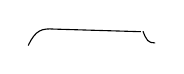
\begin{tikzpicture}[x=.55cm,y=.55cm,baseline=-.2ex]\draw (-.15,-.3) .. controls (.02,.06) and (.16,.1) .. (.45,.08)--(2.45,.02);\draw (2.5,.03) .. controls (2.58,-.18) and (2.62,-.24) .. (2.78,-.24);\end{tikzpicture}}} Elle existe sss $A$ est associative, resp. unitaire resp. commutative. Quand ces conditions sont satisfaites simultanément, on a donc un schéma en \deleted{groupes}\inserted{\handwritten{monoïdes}} affine sur $k$, qui permet de réconstituer la situation. - Si on a de même $\unsure{\deleted{F}C|\mathbb{C}}',F'$ sur le même $k$, \deleted{avec un $\otimes$,} alors les foncteurs $G:C\handwritten{\to} C'$ compatibles avec $F,F'$ correspondent exactement aux hom. de $k$-algèbre top $U'\handwritten{\to}U$, ou de $k$-coalgèbres $A\handwritten{\to}A'$. Si $\unsure{\deleted{F}C|\mathbb{C}}$ et $C'$ sont munis de structures bilinéaires $\otimes\unsure{\deleted{x}\handwritten{/}|\deleted{t}\handwritten{/}|\deleted{,}}\otimes$, alors le foncteur $G$ est un $\otimes$-foncteur avec un isomorphisme $c$ tra\deleted{e}nsformé par $F'$ en $\mathrm{id}$ (ce qui suffit à \deleted{le} caractériser\inserted{\handwritten{$c$\begin{tikzpicture}[x=.45cm,y=.45cm,baseline=-.2ex]\draw (0,-.35) .. controls (.02,-.04) and (.08,.1) .. (.3,.14)--(.7,.16) .. controls (.88,.18) and (.94,.32) .. (.95,.58);\end{tikzpicture}}} alors) sss $U'\handwritten{\to}U$ est compatible avec les diagonales i.e. $A\handwritten{\to}A'$ est compatible avec les mu\deleted{t}\handwritten{l}\deleted{l}\handwritten{t}iplications. Les éventuelles structures supplémentaires a)\deleted{, b)} ou c) sont respectées automatiquement,\inserted{\handwritten{pour b) il faut supposer \unsure{compatibilité|compatiblté} aux augm de $U$ resp. aux unités de $A,A'$}}

\margin{généraliser au moins partiellement au cas d'un $k$ qui n'est pas un corps}

\margin{\handwritten{relations entre loi $\check{X}$ et \unsure{antipodisme|antipodismes} sur $U$ resp. $A$}\figure{\begin{tikzpicture}[baseline]
\draw (0,0) .. controls (.35,.6) and (1.35,.35) .. (1.7,1.1) .. controls (1.9,1.45) and (1.65,1.65) .. (1.7,2.05) .. controls (1.7,2.7) and (1.4,3.05) .. (1,3.2) .. controls (.5,3) and (.1,2.55) .. (-.3,2.25);
\draw (1.76,1.5)--(2.7,1.5);
\end{tikzpicture}}}

\figure{\begin{tikzpicture}[baseline]
\draw (0,0)--(0,1.6);
\end{tikzpicture}}
\handwritten{Dire \inserted{\unsure{de|autre}} que les endom. de $F$ compatibles avec $c=\mathrm{id}$ sont les $g\in U$ tels que $\Delta(g)=g\otimes g$; si on veut respecter la donnée de l'unité de $(\underline{C},\unsure{\otimes|\omega})$, il faut de plus exiger $\epsilon(g)=1$, i.e. $g$ est un hom unitaire $A\to k$}

7) U\deleted{n}n exemple. On prend pour $C$ la catégorie des modules gradué\deleted{\unsure{e|s}}s sur un anneau comm\deleted{y}u\deleted{c}tatif $\unsure{\deleted{A}k|\mathbb{k}}$, avec le produit tensoriel gradué ordinaire et pour unité le module $\unsure{\deleted{A}k|\mathbb{k}}_s$ gradué par le degré zéro, donnée\deleted{s dt} de $u$ et $v$ comme d'habitude, ainsi que $\handwritten{\phi}$ (associativité) et $\handwritten{\psi}$ (commutativité). Tous les axiomes du nº1 sont vérifiés, et le foncteur oubli (avec $c=\mathrm{id}$) estrun $\otimes$-foncteur respectant toutes les données a)b)c). Donc si $k$ est
